\section{Ontology-based Streaming Data Access}
\label{approach}
% lightweight description, architecture
% include graphic
% contributions

Querying streaming data and ontology-based access to stored data sources have already been studied by the research
community and concrete proposals and software have been produced to deal with them. However there is still no bridging
solution that allows connecting these technologies coherently in order to answer the requirements of i) establishing
mappings between ontological models and streaming data source schemas, and ii) accessing streaming data sources through
queries over ontology models.

%\begin{itemize}
%\item establishing mappings between global ontological models and streaming data source schemas.
%\item accessing streaming data sources through queries over ontology global models.
%\item integrating streaming and stored data sources through an ontological unified view.
%\item combining data from event-based streams and/or sensor networks acquisitional streams considering time and tuple windows.
%\item considering quality-of-service requirements for query optimisation and source selection during the integration.
%\end{itemize}

\begin{figure}[here]
\vspace{-20pt} \hspace{20pt}
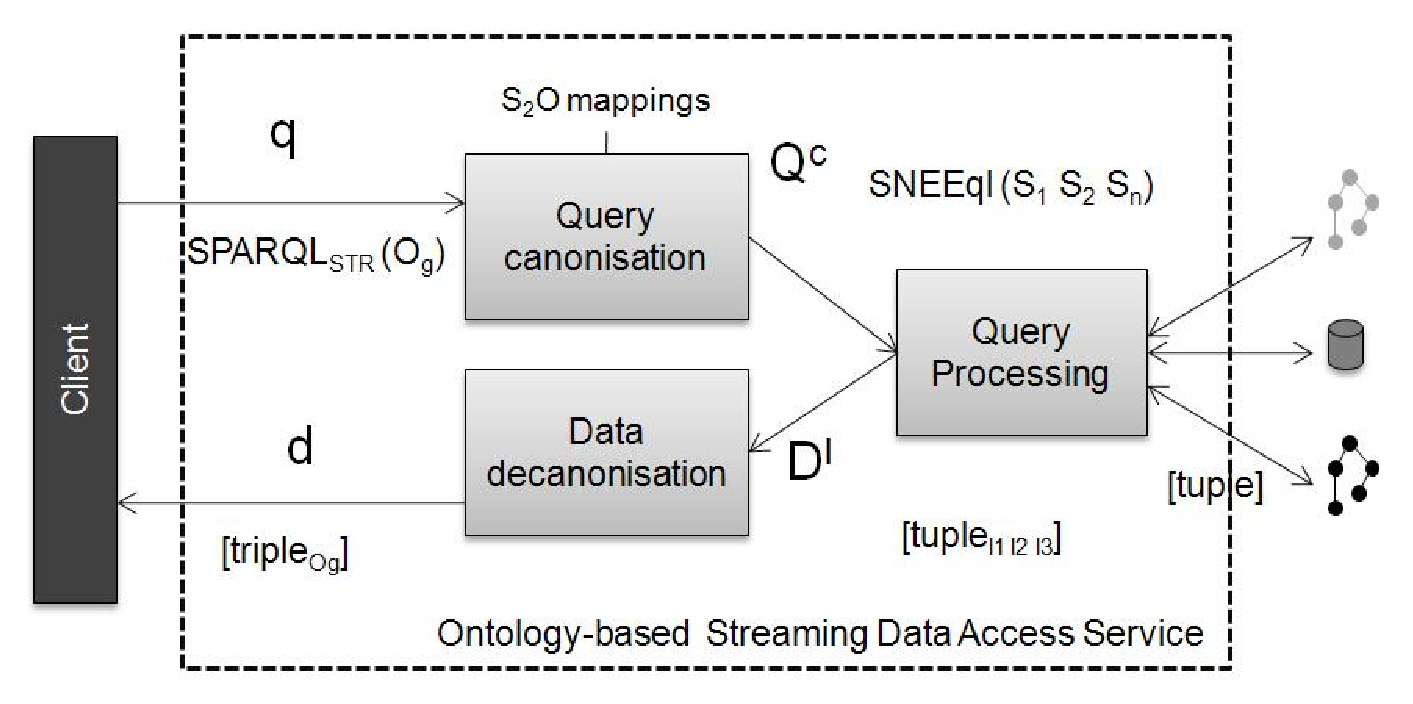
\includegraphics[width=8 cm]{img/approach}
\vspace{-10pt} \caption{Ontology-based Streaming Data Access service} \label{fig:SemanticIntegrator} \vspace{-10pt}
\end{figure}

Our approach consists in creating an Ontology-based Streaming Data Access service, depicted in Fig~\ref{fig:SemanticIntegrator}.\ %  that can receive requests over an ontological view and transforms them into queries for acquisitional or event-based stream sources or stored sources. The results of these queries can be integrated following a query plan and returned as RDF triples in terms of the global ontology. The approach is depicted in Fig ~\ref{fig:SemanticIntegrator}.
The service receives queries specified in terms of the classes and properties\footnote{We use the OWL nomenclature of
classes and object and datatype properties for naming ontology elements.} of the ontology using extensions of SPARQL
that support operators over RDF streams and windows (\sparqlstr, see the Streaming Extensions to SPARQL section). %\ref{streamingsparqlsyntax}). 
Then in order to transform the query in terms of the ontology into queries in terms of the sources, a set of mappings must be
specified. These mappings are based on the \rtwoo\ mapping language, which has been extended to support  streaming
queries and data, most notably window and stream operators (see the Streaming Extensions to \rtwoo\ section).%~  Section \ref{streamingr2osyntax}). 
This transformation process is called \textit{query canonisation}, and the target is a continuous query language (e.g. SNEEql), that is
expressive enough to deal with both streaming and stored sources, and to apply window, aggregates and window-to-stream
operations.

After the continuous query has been generated, the query processing phase starts, and the processor will deploy distributed query processing techniques~\cite{Kossmann_00} to extract the relevant data from the sources and perform the required joins, etc.\ %creating a query plan that indicates how the sources will be accessed and how the data will be joined and combined using the available operators\cite{Kossmann_00}.
%
Note that the execution in sources such as sensor networks may include in-network query processing, pull or push based data delivery and other data source specific settings. The result of the query processing will be a set of tuples that will be passed to a \textit{data decanonisation} process, which will transform these tuples to ontology instances.

As it can be seen, this approach requires several contributions and extensions to the existing technologies for continuous data querying, ontology-based data access and SPARQL query processing. This paper focuses on a first stage that includes the process of transforming the SPARQL extended queries into queries over the streaming data sources using a language such as SNEEql as the target. In the next sections a description of the query and mapping extensions syntax and semantics will be detailed, and afterwards we will provide results of an implementation of this approach.
